
\documentclass[letterpaper,times]{IONconf/IONconf}

\usepackage{amsmath}
\usepackage{graphicx}
\usepackage{multirow}
\usepackage{float}
\usepackage[ruled,vlined]{algorithm2e}

\title{On SBAS Authentication with OTAR Schemes}
\author{Jason Anderson, Sherman Lo, Andrew Neish, Todd Walter}

\begin{document}

\maketitle

\section{Full Stack Simulation and KPIs}

\begin{itemize}
	\item Discuss methodology of monte-carlo simulation
	\item Discuss Figure \ref{fig:time-of-first-fix-mc}
	\item Availability
	\item Continuity
\end{itemize}

\begin{figure}[H]
	\centering
	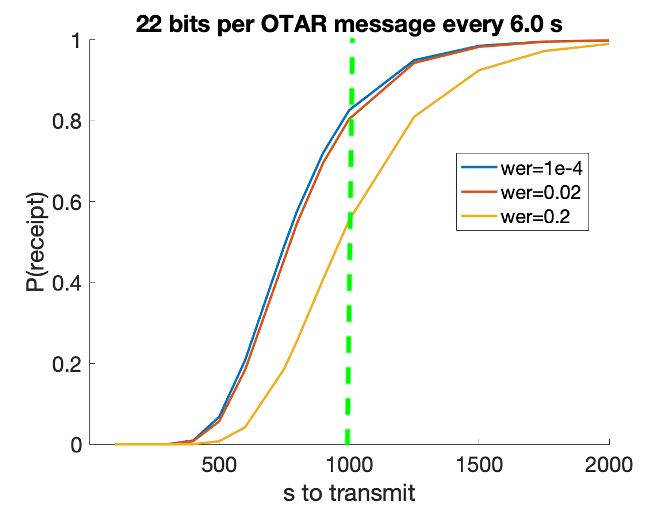
\includegraphics[width=0.4\linewidth]{fig/integrated_mc.png}
	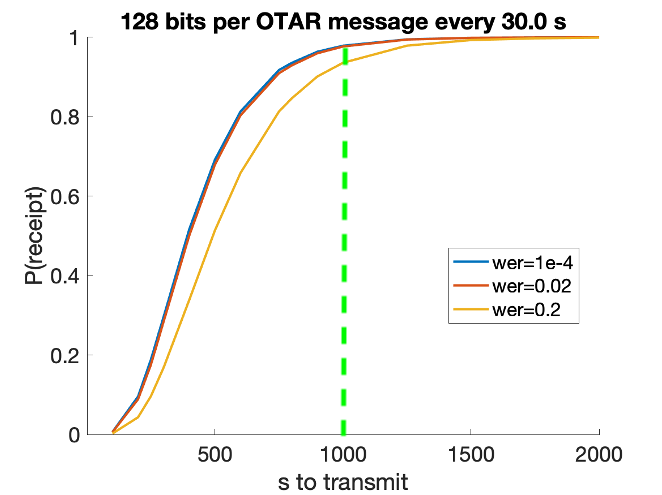
\includegraphics[width=0.4\linewidth]{fig/modular_mc.png}
	\caption{Comparison of time-of-first-fix of spare-bit approach (left) and modular approach (right) via monte carlo methods.}
	\label{fig:time-of-first-fix-mc}
\end{figure}

\section{Loose-time Synchronization and Operational Procedures}

\subsection{TESLA Timing Synchronization and Replay Attacks}
\begin{itemize}
	\item How TESLA requires time sync and therefore SBAS is vulnerable
	\item The worst Replay Attack
\end{itemize}

\subsection{Time Sync Option A: Reliance on external connection}

To verify that the timing hasn't been hacked
\begin{itemize}
	\item Discussion of allowing external connection
	\item Discussion of allowing only {\em external broadcast} connection
\end{itemize}

\subsection{Option B: Reliance on exclusive receiver clock}

Primary reference \cite{time_sync_paper}

To verify that the timing hasn't been hacked
\begin{itemize}
	\item Minimum calibration requirement given clock drift and GPS and SBAS time sync fusion
	\item machine state time procedures
	\item tie to periodic maintenance
\end{itemize}

\section{Remaining Work}

Scheme extendable to any broadcast only connection (e.g., having traffic lights broadcast their state (e.g., red, green) without spoofing problem)

\section*{Alternative Design}

\begin{table}[H]
\center
\begin{tabular}{|c|c|c|c|c|} \hline
	Preamble & MT & Cipher Text Meta Data & Cipher Text & CRC \\ \hline
	4 & 6 & 24 & 192 & 24 \\ \hline
\end{tabular}
\caption{Bit allocation proposed for MT 51 at 250 bits per message. Table \ref{tab: meta-data table} providers greater detail of the ciphertext metadata.}
\label{tab: high-level table1}
\end{table}

\begin{table}[H]
\center
\begin{tabular}{|c|c|l|} \hline
	\multicolumn{3}{|c|}{Ciphertext Meta Data} \\ \hline
	Section & Bits & \multicolumn{1}{|c|}{Value} \\ \hline
	\multirow{4}{*}{Germane Key Level} & \multirow{4}{*}{2} & 0 - Spare \\ 
	& & 1 - ECDSA AES key to decrypt Level 1 ECDSA Public Key \\
	& & 2 - ECDSA Level 2 Public Key \\
	& & 3 - TESLA Hash Path End Hash Point \\ \hline
	Germane Key Expiration & 10 & GPS Week and Time of Week of Germane Key Expiration \\ \hline
	\multirow{4}{*}{Cipher Text Type} & \multirow{4}{*}{2} & 0 - Public Key, AES Decryption Key, or Hash Point Root \\
	& & 1 - Authenticating cipher text derived from the Authenticating Key \\ 
	& & 2 - Spare \\ 
	& & 3 - Spare \\ \hline
	Cipher text Page Number & 4 & The Ordered Section of Germane cipher text - max 16 with 4 bits\\ \hline
	Next or Current Key & 1 & Either next key or current key \\ \hline
	Spare & 5 & \\ \hline
	Sum Total & 24 & \\ \hline
\end{tabular}
\caption{Bit allocation of ciphertext metadata. To distinguish the key updated with a specific MT51 and the key used to authenticate that MT51, we call the key associated with the MT51-delivered ciphertext the Germane Key and the key used to authenticate that delivered key the Authenticating Key.}
\label{tab: meta-data table1}
\end{table}

\bibliographystyle{ieeetr}
\bibliography{references}

\end{document}
